\documentclass[aps,prl,reprint,amsmath,amssymb]{revtex4-1}

% define variable that compiles the main text (as opposed to SI text)
\newcommand*{\MAINTEXT}{}

\usepackage{epsfig,color,graphicx}
\begin{document}
\newcommand{\Ang}{\ensuremath{\mathring{\text{A}}}}
\newcommand{\ltwid}{\mathrel{\raise.3ex\hbox{$<$\kern-.75em\lower1ex\hbox{$\sim$}}}}
\newcommand{\gtwid}{\mathrel{\raise.3ex\hbox{$>$\kern-.75em\lower1ex\hbox{$\sim$}}}}
\newcommand{\bra}{\langle}
\newcommand{\ket}{\rangle}
%\newcommand{\sill}{\psi_\mathrm{SILL}}
\newcommand{\sill}{\psi}
\newcommand{\trace}{{\rm Tr}}
\newcommand{\ntilde}{\tilde{n}}
\newcommand{\stilde}{\tilde{s}}
\newcommand{\atilde}{\tilde{\alpha}}
\newcommand{\new}{\color{red}}
\newcommand{\old}{\color{black}}
\newcommand{\bea}{\begin{eqnarray}}
\newcommand{\eea}{\end{eqnarray}}
\def\nn{\nonumber\\}

\bibliographystyle{apsrev}

\ifdefined\MAINTEXT
\else
	\clearpage
	%\widetext
	\setcounter{figure}{0}
	\setcounter{page}{1}
	\renewcommand{\thefigure}{S\arabic{figure}}
\fi

\title{
\ifdefined\MAINTEXT
\else
Supplementary Information: \\
\fi
Contribution of the covalent component of the hydrogen-bond network to the properties of liquid water
}

\author{Yifei Shi}
\author{Hayden Scheiber}
\author{Rustam Z. Khaliullin}
\email{rustam.khaliullin@mcgill.ca}
\affiliation{Department of Chemistry, McGill University, 801 Sherbrooke St. West, Montreal, QC H3A 0B8, Canada}

\date{\today}

\ifdefined\MAINTEXT

\begin{abstract}
Many remarkable properties of liquid water originate from the ability of water molecules to form hydrogen bond, which is a combination of electrostatic, induction, dispersion and covalent interactions. 
In this work, we developed an ab initio molecular dynamics method that enabled us to switch off the covalent component of interactions between water molecules in simulations. 
We show that for room-temperature liquid water, a seemingly small amount of electron transfer has a profound/spectacular effect on observable properties of liquid water. 
In particular, the tetrahedronal structure, O-H stretch mode and viscosity are all significantly determined by covalent interactions.
%RZK: many unique structural characteristics, spectroscopic features, and properties as a solvent are to a large extent determined by covalent interactions.
\end{abstract}
\maketitle

\section{Introduction} 

Detailed understanding of the physical nature of hydrogen bonding (HB) between molecules in water is essential for unraveling origins of unique physical and chemical properties of this ubiquitous and important liquid. 
Since the dawn of quantum mechanics, it has been known that hydrogen bonding is a complex phenomenon that arises from the interplay of several distinct effects: interaction between molecules’ permanent multipoles (dipoles, quadrupoles, etc.), polarization, dispersion, and orbital donor-acceptor interactions~\cite{eisenberg2005structure}.

Donor-acceptor interaction leads to the transfer of the electron density between molecules and, therefore, is called the charge-transfer or covalent component of HB. 
The concept of covalent interactions in HB is tremendously useful in chemistry 
%[and is deeply embedded into the everyday chemistry jargon/language. It helps] 
as it helps explain, to name only few, water's unique properties as a solvent, its ability to catalyze a wide variety of chemical processes, and strong cooperativity between hydrogen bonds in systems ranging from nanodroplets to solvated biomolecules. 
From the theoretical standpoint, the covalent component of HB has attracted significant attention because of its purely quantum mechanical nature, which, unlike electrostatic and dispersion interactions, is hard to describe with simple analytical potentials~\cite{ZZZ}.

% ZZZ: NBO - remove abbreviation. Check AIMD, MD, ALMO, DFT,

Recent developments in energy decomposition techniques based on accurate electronic structure methods have helped make substantial progress towards quantifying the individual contributions of various physical effects to the HB energy in small water clusters. 
However, the extent of intermolecular charge transfer in HB has remained the last unresolved issue until recently~\cite{isaacs1999covalency,ghanty2000hydrogen,stone2017natural}. 
Natural bond orbital analysis\cite{weinhold1998natural} and natural energy decomposition analysis \cite{glendening1994natural} have suggested that charge transfer is the major component of HB~\cite{schenter1996natural,glendening2005natural,weinhold2005resonance} because, if charge transfer is neglected, these methods show no binding at the water-dimer equilibrium geometry. 
After a debate spanning several decades, it has been argued that natural bond orbital analysis is not optimal for weak interactions~\cite{stone2017natural}. 
It appears that the covalent component of HB is better described by early decomposition methods~\cite{kitaura1976new,bagus1984new,bagus1992decomposition,stevens1987frozen,chen1996energy,ZZZ-SAPT} as well as their modern variants~\cite{mo2000energy,misquitta2003dispersion,khaliullin2007unravelling}. 
According to these methods, charge transfer contributes only around 20\% to the overall binding energy between water molecules in small clusters \cite{stevens1987frozen,chen1996energy,piquemal2005csov,khaliullin2009electron,cobar2012examination}, in agreement with chemists' long-held intuitive view of HB.

While energy decomposition methods have helped understand the importance of the charge-transfer for the binding strength in gas-phase water clusters little [RZK nothing?] is known about the contribution of the covalent component of HB to the \emph{observed} properties of liquid water. 
A great fundamental importance of studying covalency of HB has been pointed in several works that  noted a deep connection between the covalent interactions and features of the X-ray absorption~\cite{NatureComm2013}, infrared~\cite{JPCL2013}, and nuclear magnetic resonance~\cite{NatureComm2015} spectra of liquid water. 
In this work, we extended a recently developed energy decomposition method for periodic systems~\cite{Khaliullin2013JCTC} to perform an unprecedented \emph{ab initio} molecular dynamics study that measures quantitatively the contribution of the covalent component of HB to the structural, dynamical and spectroscopic properties of liquid water at ambient conditions. 
Our results show that a seemingly insignificant covalent component of HB is defining of the properties of liquid water. 
%[has a profound effect on the properties of water].

%In this work, we combined \emph{ab initio} molecular dynamics with a recently developed energy decomposition method for periodic systems~\cite{Khaliullin2013JCTC} to perform an unprecedented computational study that measures quantitatively the contribution of the covalent component of hydrogen bonding to the structural, dynamical and spectroscopic properties of liquid water at ambient conditions. 
%Our results show that a seemingly insignificant covalent component of HB is defining of the properties of liquid water. %[has a profound effect on the properties of water].

\section{Methods}

To quantify the influence of the covalent component of HB on the observed properties of liquid water we compared the properties calculated with \emph{ab initio} molecular dynamics (AIMD) using two different models. 
The first model model incorporates the intermolecular covalency fully whereas the second removes it completely.

The first model is the conventional Kohn-Sham density functional theory (DFT), in which electrons of a water molecule delocalize over all neighbors. 
This model is known to reproduce properties of liquid water reliably, in semi-quantitative agreement with experimental measurements. 
%The quality of the simulations was verified by comparing the results to the experimentally available data. 
In this work, this model is referred to as delocalized-electron, reference, or realistic model. 
% Agreement is semiquantitative

The second model is a constrained DFT method based on absolutely localized molecular orbitals (ALMO)~\cite{khaliullin2006efficient}. 
Unlike conventional DFT, ALMO DFT~\cite{Khaliullin2013JCTC} is able to confine each electron strictly to its own molecule and therefore completely remove the covalent component from intermolecular bonding. 
Mathematically, this is achieved by expanding Kohn-Sham molecular orbitals \emph{only} in terms of the atomic orbitals of the same molecules~\cite{gian,khaliullin2006efficient, blw}. 
Such molecular orbitals are called absolutely localized because they are localized on molecules in the same sense as atomic orbitals are localized on atoms. 
To shorten the discussion, intermolecular interaction without covalent component are referred to as \emph{devalent} interactions and the ALMO-based model is called localized-electron or \emph{devalent} model. 
It is important to note that this model retains all other physical effects, including the covalent component of \emph{intramolecular} OH bonds. %were variationally optimized on each AIMD each step to find the electronic ground state of the system.
To ensure that the covalent component of intermolecular bonding is removed accurately we performed several tests described in the Supplementary Information.

To keep electrons absolutely localized in a course of AIMD simulations, we extended the recently developed ALMO DFT method for  condensed molecular systems~\cite{Khaliullin2013JCTC} so that the atomic forces can be computed analytically from the ALMO DFT energies (see Supplementary Information).

All AIMD simulations, with delocalized and localized molecular orbitals, were performed using the dispersion-corrected~\cite{grimme2010consistent} BLYP exchange-correlation functional~\cite{becke1988density} and TZV2P basis set~\cite{vandevondele2007gaussian}. 
The temperature of simulations was set to 298~K. 
The size of a periodic cubic simulation box was fixed to reproduce the experimental 0.997~g$\cdot$cm$^{-3}$ density of ambient liquid water. 
Since removing intermolecular covalency can affect the density, we also performed a set of simulations for a system, which density was adjusted to 1~atm using constant pressure AIMD. 
The length of the AIMD simulations was chosen to obtain statistically meaningful results. 
A detailed description of the calculations is presented in the Supplementary Information.

%RZK: \new Temperature and potential are ``two peas in a pod''. Removing covalent interactions weakens HBs. Can we recover properties of room-temperature liquid water using the devalent model at lower temperature? The same question can be asked another way: is devalent room-temperature water completely equivalent to high-temperature covalent water? We know the exact contribution of covalency to the binding energy of molecules. How much the temperature should be adjusted to keep the average Boltzmann weights the same?\old

At this point, it is appropriate/important to comment on the ability of the reference model to reproduce properties of real water. 
[GGA is known to underestimates the energy gap slightly. 
As a result they overestimate the electron delocalization, overbinds molecules, produces RDF with sharper peaks than those derived in X-ray scattering experiments. 
Underestimated diffusion constant, overestimated viscosity. 
However, for all calculated properties the imperfections of the reference model are far less significant than the changes induced by neglecting intermolecular covalency. 
This is the main reason we are confident that our devalent model is an accurate depiction of the contribution of the covalent component to the properties .]


\section{Results and discussion}

Variational principle of quantum mechanics guarantees that removing covalent interactions weakens intermolecular bonding. 
ALMO-based decomposition energy analysis predicts that, in a water dimer, the transfer of 0.27\% of an electron contributes  7.0~kJ$\cdot$mol$^{-1}$ (37\%) to the overall stabilization of the hydrogen bond at equilibrium geometry, in agreement with earlier reports~\cite{stevens1987frozen,chen1996energy,piquemal2005csov,RZK-khaliullin2009dimer}. 
This contribution is higher in the \emph{cooperative} HB network of liquid water at ambient conditions: 1.1\% of electron and 19 ~kJ$\cdot$mol$^{-1}$ per hydrogen bond, in agreement with our previous study \cite{kuhne2014nature}.

\textbf{Molecular structure.} The covalent component of weak intermolecular bonds has only a minor effect on the shape of water molecules. 
The average length of intramolecular OH bond changes from [RZK the values are wrong- we talk about INTRAmolecular bonds here] \new2.33\old~\Ang\ in the realistic model to \new 2.75\old~\Ang\ in the devalent model of water. 
At the same time, the average intramolecular HOH angle changes from 105.5 degrees to 104.3 degrees, becoming closer to the value calculated for the 298~K gas phase water molecule.

\begin{figure}
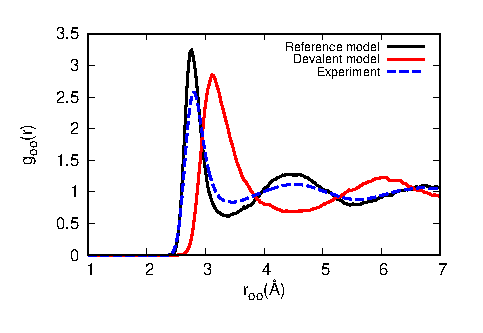
\includegraphics[width=0.5\textwidth]{new_rdf}
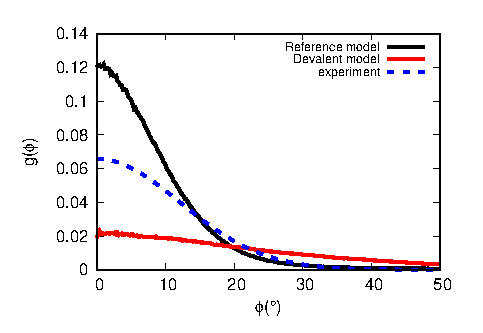
\includegraphics[width=0.5\textwidth]{new_adf}
\caption{A. Oxygen-oxygen radial distribution function. B. Angular distribution of the H--O$\cdots$O angle computed for hydrogens within 2.3~\Ang\ from a reference molecule.} \label{Fig:RDF}
%RZK: Describe the normalization of the ADF
%RZK: It makes sense to keep the angular distribution only if we can compare it to the experimental curve. Otherwise, we have SPD. Experimental curves available. See, for example, http://pubs.acs.org/doi/pdf/10.1021/ct3001848 Figure 2.
\end{figure}

%RZK: Suggested color coding throughout the manuscript: realistic - black, devalent - red, experiment - black dash, vapor - blue, devalent NPT - blue (these colors make it easier for color blind persons to read figures and at the same time minimize the publication cost). Legends throughout: ``Realistic model'', ``Devalent model'', ``Experiment''. 
%RZK: Decrease panel height. See figure guidlines for Nature Chemistry.

The effect of the covalency on the structure of the HB network is far more pronounced. 
The oxygen-oxygen radial distribution function (RDF) in Figure~\ref{Fig:RDF}A shows that weaker devalent interactions lead to the considerable expansion of the first coordination shell of a water molecule from the ``realistic'' average of 2.8~\Ang\ to 3.1~\Ang. 
The shift of the first-shell peak is accompanied by its broadening that is indicative of a wider variety of configurations available to devalent HBs.

These dramatic changes in the structure of the HB network are consistent with the decrease in the HB strength. 
It is remarkable, however, that the remaining components of HB -- permanent electrostatic, polarization and dispersion -- are sufficiently strong to retain several characteristic structural features of the network: well-defined coordination shells and directional HBs~\cite{arunan2011definition}.
%
%Arunan E, Desiraju G R, Klein R A, Sadlej, ScheinerS, Alkorta I, Clary D C, Crabtree R H, Dannenberg J J,Hobza P, Kjaergaard H G, Legon A C, Mennucci B andNesbitt D J 2011 Pure Appl. Chem. 83 1619.
%
Indeed the second coordination peak in the RDF of the devalent model remains clearly visible though shifted to higher distances. 
The distribution of HB angles also still has a maximum at 0$^\circ$ despite becoming broader (Figure~\ref{Fig:RDF}B).

The structure of the HB network for both models can also be illustrated with the spatial distribution of oxygen atoms around a reference water molecule (see cross sections in Figure~\ref{Fig:SDF}). 
It is clear that the distorted tetrahedral structure of liquid water is retained without the covalent component (cf. Figure~\ref{Fig:SDF}A and \ref{Fig:SDF}AB), indicating that permanent electrostatic and polarization interactions tend to orient water molecules the same way as the covalent interaction. 
%[RZK: Notion that covalency is responsible for directional character of HB is not entirely correct.] 
For comparison, if a model retains only dispersion interactions and short-distance repulsion, represented by the Lennard-Jones potential, the HB becomes truly non-directional with uniform angular distribution (Figure~\ref{Fig:SDF}C). 
That is why, permanent electrostatics is widely recognized as the key component of interaction between water molecules and is included in all analytical molecular mechanics models of water. 
% RZK: move to conclusions?
On the other hand, the equally strong covalent component is neglected in these models and instead compensated by fine-tuning permanent atomic charges (see Figure~\ref{Fig:SDF}D, for example). 
While such models are very successful in reproducing a wide variety of properties of aqueous systems~\cite{Vega2011} [it has been argued that] the failure to include covalent effects properly limits their applicability to RZK~\cite{, RZK-weinhold}. % RZK: only if covalent interactions are substantially different from fixed electrostatics

% RZK: Vega2011 -- DOI: 10.1039/c1cp22168j

\begin{figure*}
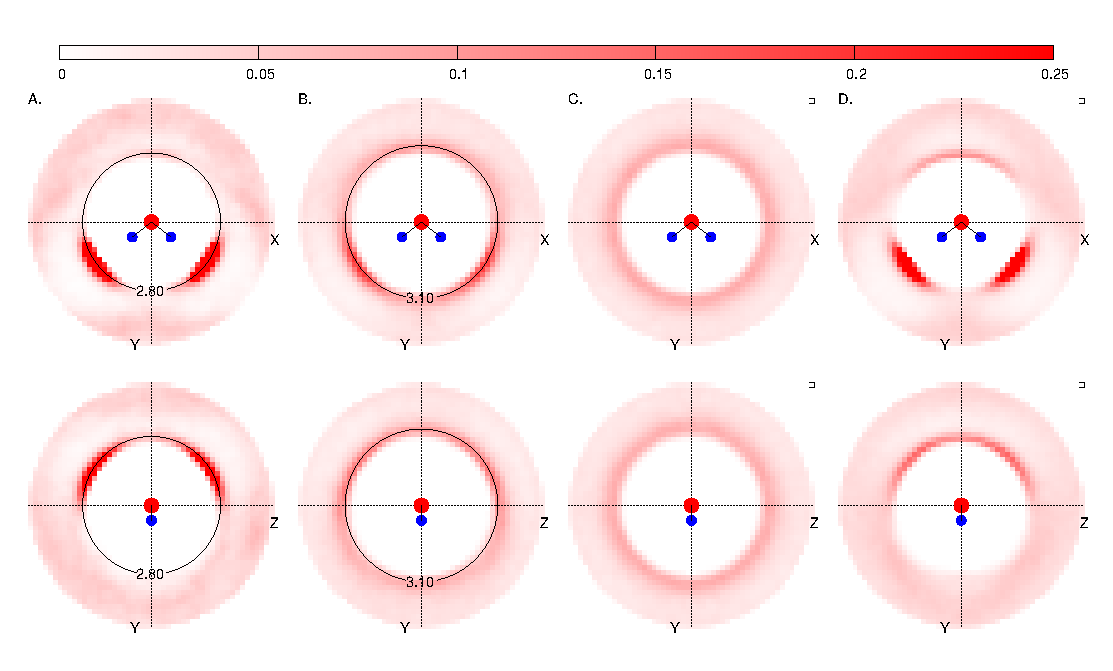
\includegraphics[width=0.9\textwidth]{SDF}
\caption{Cross sections of the spacial distribution of oxygen atoms. 
The upper panels show the cross section of the spacial distribution function in the plane of the reference water molecule, whereas the lower panels show the cross section in the plane disecting the molecule. 
A. Reference model, B. localized model, C. Modified TIP3P model that include only van der Waals interactions, D. TIP3P model~\cite{TIP3P}: electrostatic interaction between atomic point charges combined this van der Waals interactions~\cite{TIP3P}.} \label{Fig:SDF}
\end{figure*}

%RZK: It is interesting that the average intermolecular distance increases significantly when covalent component is switched off (Figure~\ref{Fig:RDF}A) while the density of both reference and devalent models is fixed to be the same. This indicates that 

\textbf{Density of liquid water.} If the density is allowed to fluctuate in a simulation while the pressure is fixed at 1~atm, the average density decreases from ZZZ~g$\cdot$cm$^{-3}$ [RZK: I do not have the NPT density] for the reference model to 0.83~g$\cdot$cm$^{-3}$ for the devalent model or by ZZZ\%. 
While this is a noticeable drop it is important to note that the devalent water is still liquid at ambient conditions because of strong electrostatic, polarization and dispersion effects. 

The ZZZ\% decrease in the density should correspond to a 6\% [RZK: check the number] elongation of intermolecular distances assuming that they all increase uniformly. Nevertheless, the position of peaks in RDF remains the same in the devalent water at two different densities (Figure~S-ZZZ). The only noticeable structural change is that peaks become slightly broader in the low-density constant-pressure model and angular distribution is slightly wider. This indicates that most molecules stay in the same position around the minimum of the potential well when the density is allowed to relax. Only a small fraction of them becomes distorted in the radial and angular directions. 

We will continue discussing properties of the \emph{fixed-density} devalent water further because all key properties obtained for the fixed-pressure model are almost the same (see Supplementary Information).

% RZK: density of butanol is 0.810, 3-Pentanone -- 0.815, 2-Octanol -- 0.824

\textbf{Infared spectrum.} Figure~\ref{Fig:IR} shows the infared (IR) spectra of the devalent and reference systems together with that of ideal water vapor at 298~K. 
The most pronounced difference in the IR spectra is in the 3000--4000~cm$^{-1}$ region of intramolecular O--H stretching bands $\nu$. 
For the devalent model, $\nu$ peaks do not exhibit the redshift and broadening characteristic to hydrogen-bonded O--H groups and clearly seen in the spectrum of the realistic model. 
Comparison of the spectra of the devalent and gas-phase models indicates that the characteristic redshift is entirely due to covalent interactions. 
Even the small amount of electron density donated from a neighbor oxygen into the antibonding orbitals localized of an intramolecular O--H bond (see Figure ZZZ in Ref.~\onlinecite{RZK-chem-eur-j-2009}) is sufficient to soften the O--H bond and thus lower its vibrational frequency by ZZZ~cm$^{-1}$. 

This primary role of the covalent component in the broadening of the $\nu$ peaks also becomes apparent. 
This broadening is normally attributed to a great variation in the strength of hydrogen bonds that leads to a great variation in the magnitude of the redshift. 
As discussed above the devalent water exhibits greater variation in the geometry of HB structures than the realistic model (compare Figure~\ref{Fig:RDF}A and~\ref{Fig:SDF}B). 
Despite this variety the $\nu$ peaks of devalent water remain very narrow indicating that without the covalent component 
the redshift is insignificant. %that the symmetric and asymmetric stretching modes become resolved in the spectrum of devalent model. 

%Since in liquid water, the shift of the centre of $\nu$ band is caused by the coupling between the O-H stretch mode and librations \cite{marechal2006hydrogen}, it then implies that this coupling is mainly through covalent interactions. 

\new 
%RZK
How do we explain the integrated intensity? It is not the same as broadening.
%However, the integrated intensity of the $\nu$ band is still $\sim$10 times larger than that of water vapor, which is generally an indication of the existence of HBs.
\old 

Unlike stretching modes, the intramolecular bending modes in the region of ZZZ~cm$^{-1}$ are unaffected by intermolecular forces and remain approximately the same for the realistic, devalent, and ideal-gas systems. It is worth noticing that the stretching and bending peaks of the devalent model do not exhibit the additional structure, which is visible in the spectra of gas-phase molecules, because the retained intermolecular forces are sufficiently strong to hinder rotations.

Another significant difference between the realistic and devalent systems is in the peaks below 1000~cm$^{-1}$, which correspond to HB stretching vibrations ($\sim$200~cm$^{-1}$ in realistic model) and molecular librations ($\sim$700~cm$^{-1}$), are shifted in the direction opposite to the intramolecular stretching modes. This is because the intermolecular bonding, unlike intramolecular bonding, becomes softer when the covalent component is switched off, in agreement with a wider variety of geometric configurations accessible in the devalent water. 

\begin{figure}
\centering
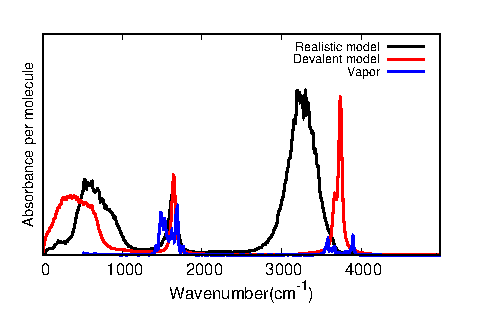
\includegraphics[width=0.5\textwidth]{new_ir}
\caption{Calculated IR spectra. The far infrared part of the spectrum for the ideal-gas system, which corresponds to rotational modes, is not shown for simplicity. 
} \label{Fig:IR}
\end{figure}

\textbf{Molecular dipole moment and dielectric constant.} Water's unique properties as a solvent are due to both the high dipole moment of its molecules and its high dielectric constant. The latter measures the ability of the molecular dipoles to reorient and stabilize ions and polar solute molecules. The experimentally measured dipole moment of a gas-phase water molecule is 1.85~D~\cite{CRC} and the dielectric constant of liquid water [RZK: at room temperature?] is the record high 78~\cite{CRC?}.

\begin{figure}
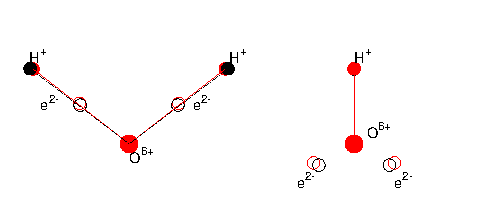
\includegraphics[width=0.5\textwidth]{acoord}
\caption{Average positions of atoms (solid circles) and Wannier centers (empty cicles) in a water molecule for the realistic (blue - ZZZ must be black) and devalent (red) models. RZK: can we add isolated molecule? Add charges to all centers: hydrogen +1, Wannier -2, Oxygen +6} \label{Fig:acoord}
\end{figure}

%RZK: CRC -- Lide, David R. (2003-06-19). CRC Handbook of Chemistry and Physics, 84th Edition. CRC Handbook. CRC Press. 9—Dipole Moments. ISBN 9780849304842.
 
Because of the continuity of the electron density the definition of molecular dipole moments in condensed phase is somewhat ambiguous. However, molecular dipoles can be estimated by assigning the electron density to molecules using the computed positions of the enters of maximally localized Wannier orbitals (Figure~\ref{Fig:acoord})~\cite{RZK}. 
The resulting dipole distribution in shown in Figure~\ref{Fig:dipoledist}. 
The average dipole moment of a water molecule is 3.09~Debye for the reference system and 2.47~Debye for the devalent system. For an isolated molecule [RZK: at zero/298~K], it is 1.96~Debye. 
Thus covalent interactions are only partially responsible for the impressive 1.13~Debye increase of the molecular dipole moment from gas to the condensed phase. 
Figure~\ref{Fig:acoord} shows that the change in the dipole moment is primarily caused by the change in the position of the lone electron pairs on the oxygen atom.
\new
RZK: how do we explain the different spread in molecular moments? In the same way we explain $\mu$?
\old

The dielectric constant can be calculated through the fluctuation of the total dipole moment\cite{neumann1983dipole,adams1981theory}:
%
\bea
\epsilon = 1+\frac{4\pi}{3V k_B T}  (  \langle |\vec{M}|^2 \rangle  - \langle |\vec{M}| \rangle ^2) \label{Eq:dielectric}
\eea
%
where $V$ and $\vec{M}$ are the volume and total dipole of the simulation box, respectively. 
The dielectric constant for the realistic model is 70, in good agreement with the experimental value of 78. 
For the devalent model, this value increases to 180.

%RZK - insert dielectric constant into the table with properties.

\begin{figure}
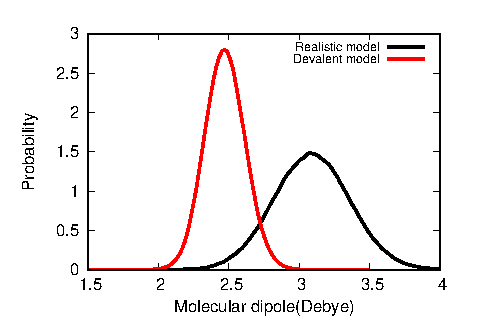
\includegraphics[width=0.4\textwidth]{new_dipole}
\caption{Distribution of dipole moments of water molecules.} \label{Fig:dipoledist}
\end{figure}

\textbf{HB network statistics and dynamics.} We show in Fig~\ref{fig:HBstat} how many HBs a molecule donate(D) or accept(A), with a geometric criterion that the H-O-O angle is smaller than 30$^{\circ}$ and the O-O distance is smaller than 3.5\Ang. 
The number of HBs is 35\% less in the localized system.

\begin{figure}
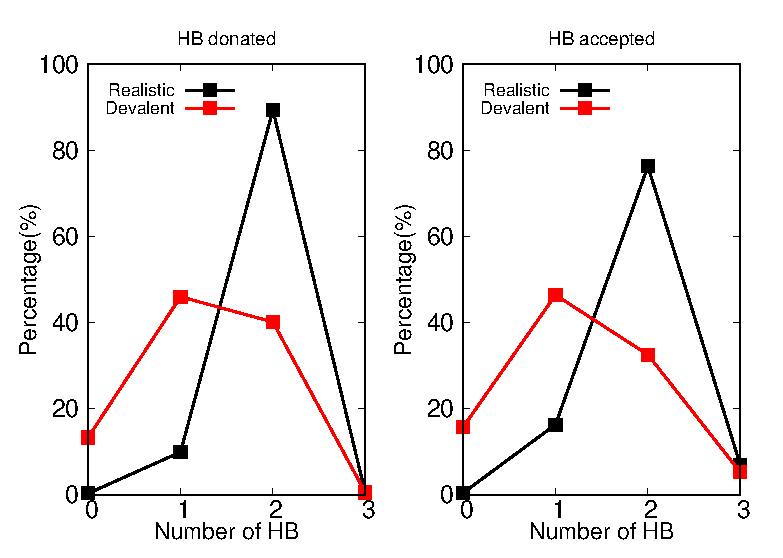
\includegraphics[width=0.4\textwidth]{new_hbstat}
\caption{HB statistics for liquid water with and without intermolecular covalency.}\label{fig:HBstat}
\end{figure}

The HB decay function $C_{HB}(\tau)$ is defined as:
\bea
C_{HB}(\tau) = \frac{\sum_{i,j}\langle \theta_{ij}(\tau)\theta_{ij}(0) \rangle}{\sum_{i,j}\langle \theta_{ij}(0) \theta_{ij}(0) \rangle} \label{Eq:HBdecay}
\eea
where $\theta_{i,j}(\tau)$ equals to 1 if there is a HB formed between molecule $i$ and $j$ through out the time period of $t=0$ to $t=\tau$. 
At large enough time it should decay exponentially, and the HB life time $\tau_{HB}$ is defined as the rate of decay: $C_{HB}(\tau) \sim e^{-\tau/\tau_{HB}}$. 
The HB decay function is shown in Fig~\ref{Fig:HBdecay}.

\begin{figure}
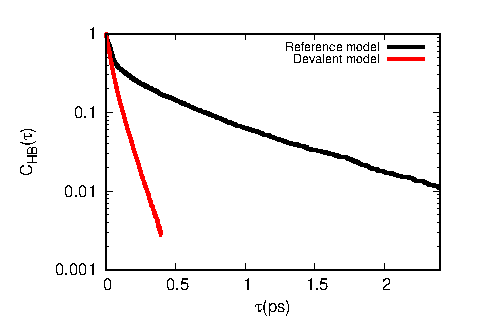
\includegraphics[width=0.4\textwidth]{new_hbdecay}
\caption{HB decay function for delocalized reference and localized system.} \label{Fig:HBdecay}
\end{figure}

The calculated HB life time for delocalized system is 0.7ps, and for localized system it becomes 0.08ps, indicating that HB are much less stable without covalent interaction.
 
 
\textbf{Diffusion constant and viscosity.} D and $\eta$ were calculated using the method of ZZZ~\cite{dunweg1993molecular}. 
The result is listed in Tab~\ref{Tab:dfs}. 
For delocalized reference the calculated viscocity is larger than the experimental value, a consequence of overestimating interaction strength in the XC functional. 
And it also implies that about 90\% of water's viscosity comes from covalency.

\begin{figure}
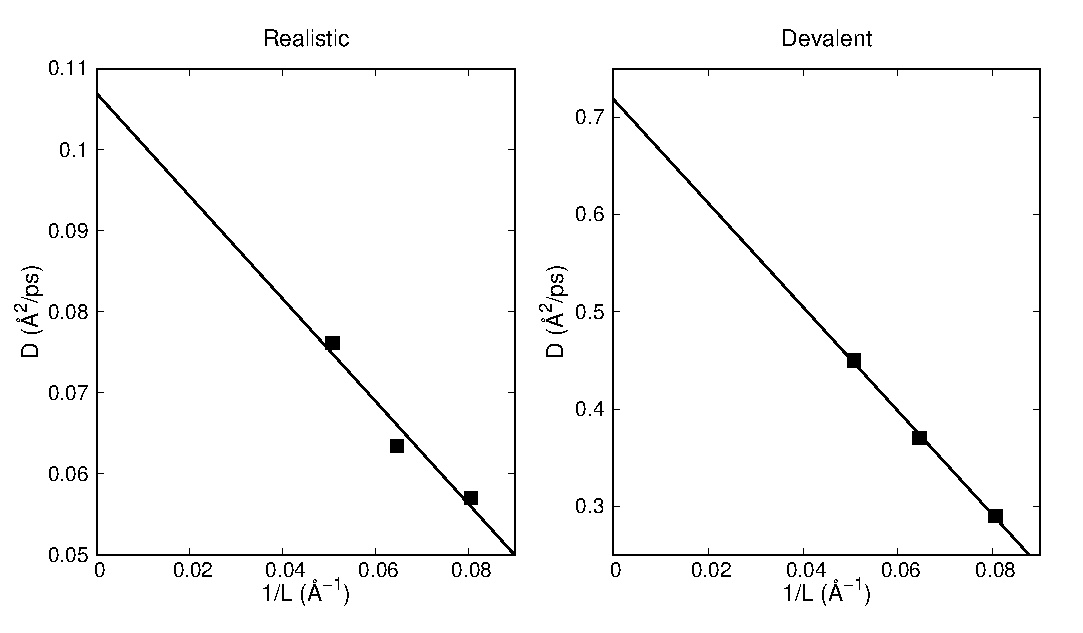
\includegraphics[width=0.5\textwidth]{msd}
\caption{Diffusion constant as a function of the system size, for 64, 125 and 256 water molecules. 
The square dots are from simulation and solid line is a linear fit.}\label{Fig:dfs}
\end{figure} 

\begin{table}
\caption{Viscosity and diffusion constant}\label{Tab:dfs}
\begin{tabular}{l*{6}{c}r}
\hline
               & $D(\Ang^2/\text{ps})$ & $\eta(\text{Pa}\cdot \text{s})$ \\
\hline
Devalent model                & 0.7188 & 3.5$\times 10^{-4}$ \\

Realistic model              & 0.1069 & 2.95$\times 10^{-3}$\\

Experimental            & 0.239  & 8.9$\times 10^{-3} $
\end{tabular}
\end{table}
 
\textbf{Conclusions.} In this work, we present the effect of the covalent interaction on observable properties of liquid water, and show that although the charge transfer energy only makes up 30\% of the total bonding energy, it plays a dominant rule in some other properties, like the OH stretch mode, viscocity, HB life time. 
And also significantly changes dipole moment, angular distribution.
 
Our result also suggest that classical models that don't take account of covalency only have limit applicability, as they fine-tune the parameters only for certain conditions.
 
Implications: shows that ALMO-based AIMD is an excellent tool for the nature of intermolecular bonding in other condensed phase systems. 
Catalysis, solvation.

\section{Detailed description of computational methods}

\textbf{ALMO DFT.} Implementation of energies and FORCES in CP2K with a quick review of its dual-basis feature.

\textbf{Settings.} All AIMD simulations were performed using the dispersion-corrected~\cite{grimme2010consistent} BLYP exchange-correlation functional~\cite{becke1988density}, large TZV2P Gaussian basis set, 320 Ry cut-off energy for the plane basis set, and GTH pseudopotentials~\cite{goedecker1996separable,krack2005pseudopotentials}. 
The size of a periodic cubic simulation box containing 125 water molecules was set to reproduce the experimental 0.997~g$\cdot$cm$^{-3}$ density of ambient liquid water. 
The temperature of simulations was set to 298~K and was controlled by a weakly-coupled canonical velocity re-scaling thermostat~\cite{bussi2007canonical} with the coupling time constant set to 300~fs. 
A short time step of 0.5~fs ensured accurate integration of the equations of the motion. 
The total length of simulations for each system was above 7~ps after a equilibrium period of 1.5 ~ps.

The properties of water including the infrared spectrum, radial distribution, dipole distribution and mean-square deviation were calculated from the MD trajectories using the TRAVIS package~\cite{brehm2012travis}.  

\section{Acknowledgments} 

The research was funded by the Natural Sciences and Engineering Research Council of Canada through the Discovery Grant. 
The authors are grateful to Compute Canada and McGill HPC Centre for computer time.

\bibliography{covalency}

\else % maintext - SI switch

\subsection{Evaluation of the diffusion constant and viscosity coefficient} 

The diffusion constant for a periodic system is known to have strong dependence on the size of the simulation box, due to the interaction of a particle with its periodic images~\cite{dunweg1993molecular}. 
And the diffusion constant obeys:
%
\bea
D(\infty) = D(L) + \frac{k_BT\zeta}{6\pi \eta L},
\eea
%
where $D(L)$ is the diffusion constant for a system of size $L$, $\eta$ is the translational shear viscosity, and $\zeta$ is a constant of 2.837. 
We calculate the diffusion constant from the mean squre deviation of the molecules, for systems of 64, 125, and 256 molecules, and find the viscosity through the dependence of $D(L)$ on $1/L$, which is shown in Fig~\ref{Fig:dfs}.

\subsection{Density dependence of localized system} 

This system will be denoted by low density localized system.

Here we present the calculation of the system at a density of the NPT ensemble at 1atm, which is 0.85g/cm$^3$. 
The O-O and O-H radial distribution function is shown in Fig~\ref{Fig:rdf_cp}. 
The position of the peak doesnot move much for the O-O distritution but the peak is more shallow for the low density system. 
O-H distance tends to be further in the low density system.

\begin{figure}
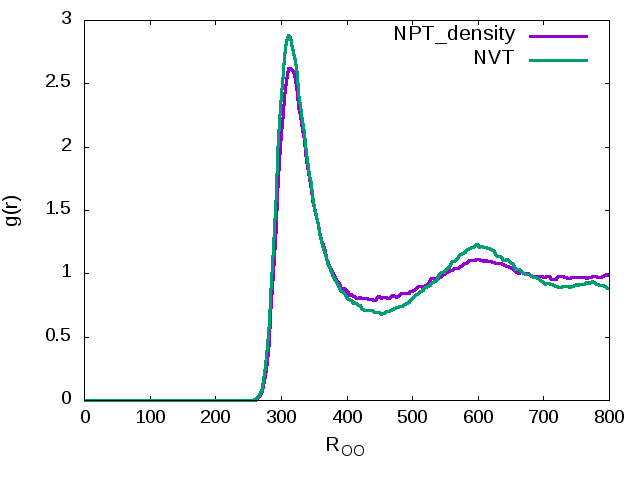
\includegraphics[width=0.45\textwidth]{rdf_NVT_CPDNVT.png}
%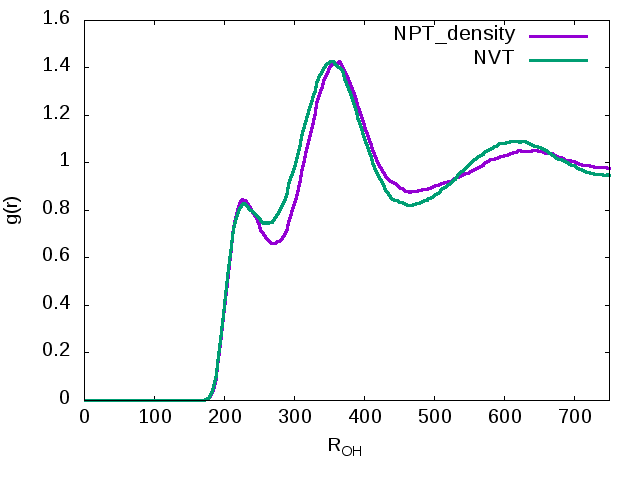
\includegraphics[width=0.45\textwidth]{rdf_OH_NVT_CPDNPT.png}
\caption{O-O and O-H radial distribution function for the 2 systems. The cutoff for the O-H distance is set to be 2.6\Ang.}\label{Fig:rdf_cp}
\end{figure} 

Then angular distribution is shown in Fig~\ref{Fig:adfcp}. 
Although the interaction for the low density system is weaker, the angular distribution is slightly more ordered. 
The IR spectrum for the 2 systems are almost identical, as shown in Fig~\ref{Fig:ir_cp}.

\begin{figure}
%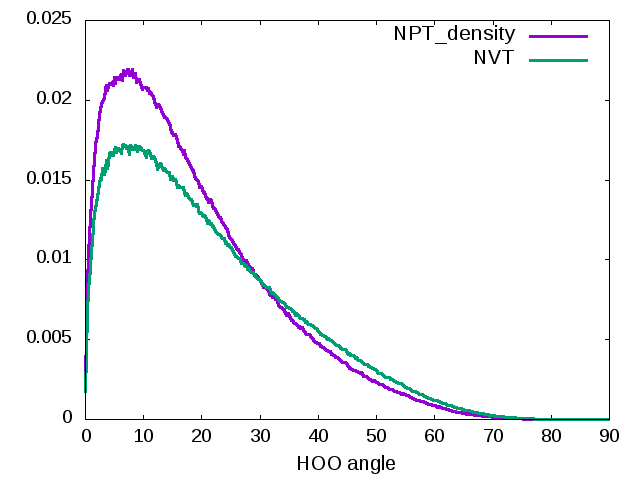
\includegraphics[width=0.45\textwidth]{angular_NVT_NPTCP}
\caption{Angular distribution function for the 2 systems.}\label{Fig:adfcp}
\end{figure} 

\begin{figure}
%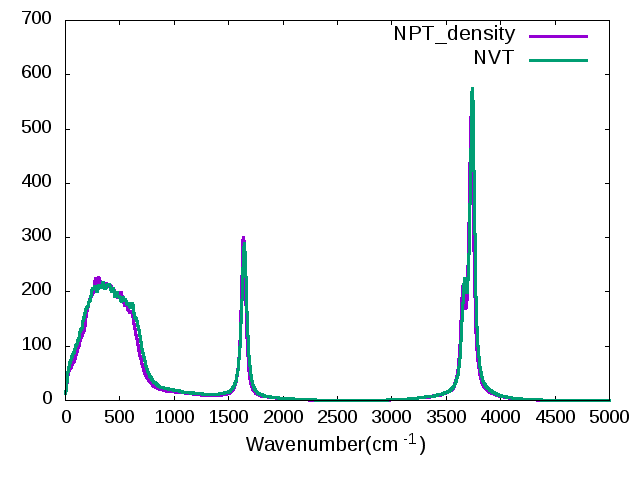
\includegraphics[width=0.45\textwidth]{ir_NVT_NPTCP}
\caption{IR spectrum for the 2 systems.}\label{Fig:ir_cp}
\end{figure} 

\subsection{Basis set dependence of the results}

It is know that a straightforward utilization of ALMOs in energy decomposition methods may underestimate charge-transfer effects especially if large basis sets are used~\cite{horn2015polarization,herbert2016}. 
This deficiency arises from the lack a well-defined separation between the polarization and charge transfer effects in the original ALMO EDA method~\cite{khaliullin2007unravelling} in the complete basis set limit. 
It has been demonstrated This problematic aspect of ALMO EDA has been recently be corrected by selecting an appropriated subset of acceptor orbitals\cite{horn2015polarization}. 
To ensure that our results are not effected by changes in the size of the basis set we re-run AIMD simulation with a larger aug-TZV2P basis set. 
ZZZ and compare the results with the calculation of TZV2P basis set, which is used otherwise in this work. 
The results are summarized in Fig~\ref{Fig:basis}.

Moreover, TZV2P basis set has been shown to give [quantitatively] accurate description of CT effect in zero-temperature water cluster. 
It is also important to note that AIMD simulations become unstable if larger basis sets (e.g. QZV) are used to model liquid water. 
This is because of frequent appearance of molecular configuration with linear dpendencies in the basis set.

\begin{figure}
%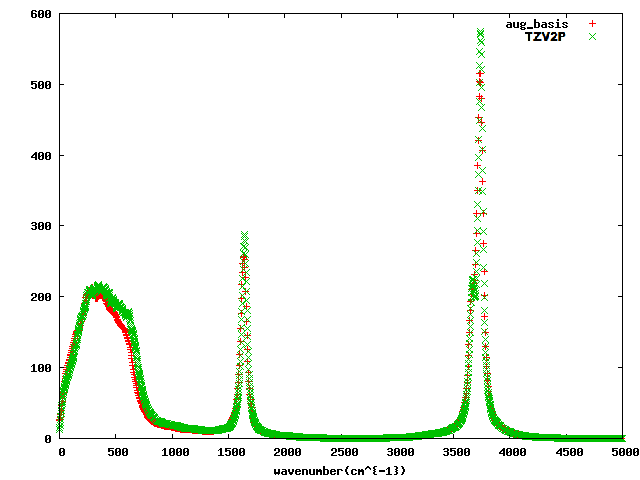
\includegraphics[width=0.35\textwidth]{aug_ir}
%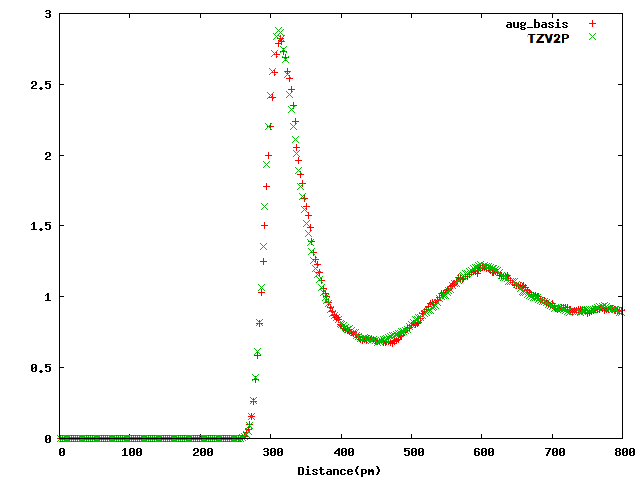
\includegraphics[width=0.35\textwidth]{aug_rdf}
\caption{IR and RDF with aug-TZV2P basis set}\label{Fig:basis}
\end{figure} 


\fi % maintext - SI switch

\end{document}
